\chapter{Analisi dei requisiti}

\section{Comunicazione}
La prima cosa che dobbiamo analizzare \`e la tipologia di messaggi che possono essere scambiati tra il gestore dei messaggi, i client e il server che gestisce i test.

Per avere un riferimento stiliamo innanzitutto un elenco dei messaggi che potrebbero essere scambiati tra il server e i client in una situazione standard.
\subsection{Esempi di messaggi che possono essere utilizzati}
\begin{itemize}
	\item Registrazione nuova postazione
	\item De-registrazione postazione
	\item Richiesta codice di accesso
	\item Invio codice di accesso
	\item Richiesta invio dati studente
	\item Invio dati studente
	\item Richiesta test da somministrare
	\item Invio contenuto del test da somministrare
	\item Invio risposte test
	\item Termine forzato del test
	\item Mostra messaggio sulla postazione
	\item Richiesta stato postazione
\end{itemize}
\subsection{Requisiti tecnici}
Per poter poter comunicare sia lato client che lato server, visto che le comunicazioni avvengono gi\`a su http o https non useremo erlang direttamente ma ci affideremo al web server Yaws \cite{web:yaws} che \`e stato implentato proprio in Erlang e che permette di inserire all'interno del codice html, in modo simile a PHP, direttamente chiamate a codice Erlang.
Saremo costretti ad adattare il codice del client e del server in modo che comunichino attraverso il nuovo gestore dei messaggi.

\section{Differenze tra le due modalit\`a}
La differenza principale, nella comunicazione tra client e server \`e che nella configurazione originale, senza il gestore dei messaggi, ogni richiesta del client viene gestita direttamente dal server che risponde, nella stessa connessione, con la pagina o il messaggio relativo.

\begin{figure}[!hbtp]
	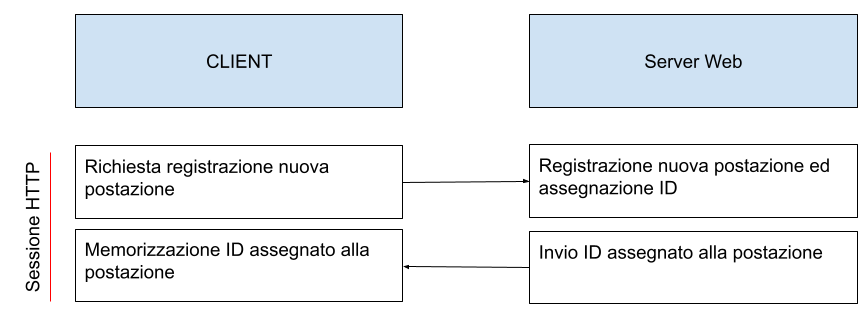
\includegraphics[width=1.0\textwidth]{figure/Disegno 003_ Esempio comunicazione senza gestore messaggi.png}
	\caption{Esempio comunicazione senza gestore messaggi}
	\label{fig:Esempio_comunicazione_senza_gestore_messaggi}
\end{figure}

Nella configurazione con il gestore dei messaggi invece la comunicazione avviene in modo asincrono. Il client fa una richiesta al gestore dei messaggi, questo risponde nella stessa comunicazione con l'ID con il quale la richiesta \`e stata memorizzata nella coda dei messaggi in modo che il client possa sapere quando la richiesta \`e stata processata.

Ad intervalli regolari il client far\`a una richiesta al gestore dei messaggi per conoscere l'esito della sua richiesta.

La comunicazione tra gestore dei messaggi e server PHP avverr\`a in modo simile.
Il gestore dei messaggi prender\`a uno dei messaggi dalla coda e si colleger\`a al server PHP. Per evitare le congestioni implementeremo un sistema che limiti il numero di processi contemporanei attivi. Se tutte le connessioni che abbiamo deciso fossero gi\`a occupate il gestore di messaggi metter\`a il messaggio di nuovo nella coda ed attendender\`a un tempo variabile prima di tentare nuovamente.

Se la connessione va a buon fine il server PHP ci risponder\`a con il risultato della richiesta. Questa verr\`a nuovamente memorizzata nella coda dei messaggi come risposta pronta per essere inviata al client corrispondente all'ID della richiesta originale.

Nel caso della comunicazione con il server avremo una comunicazione sincrona anzich\`e asincrona.

\begin{figure}[!hbtp]
	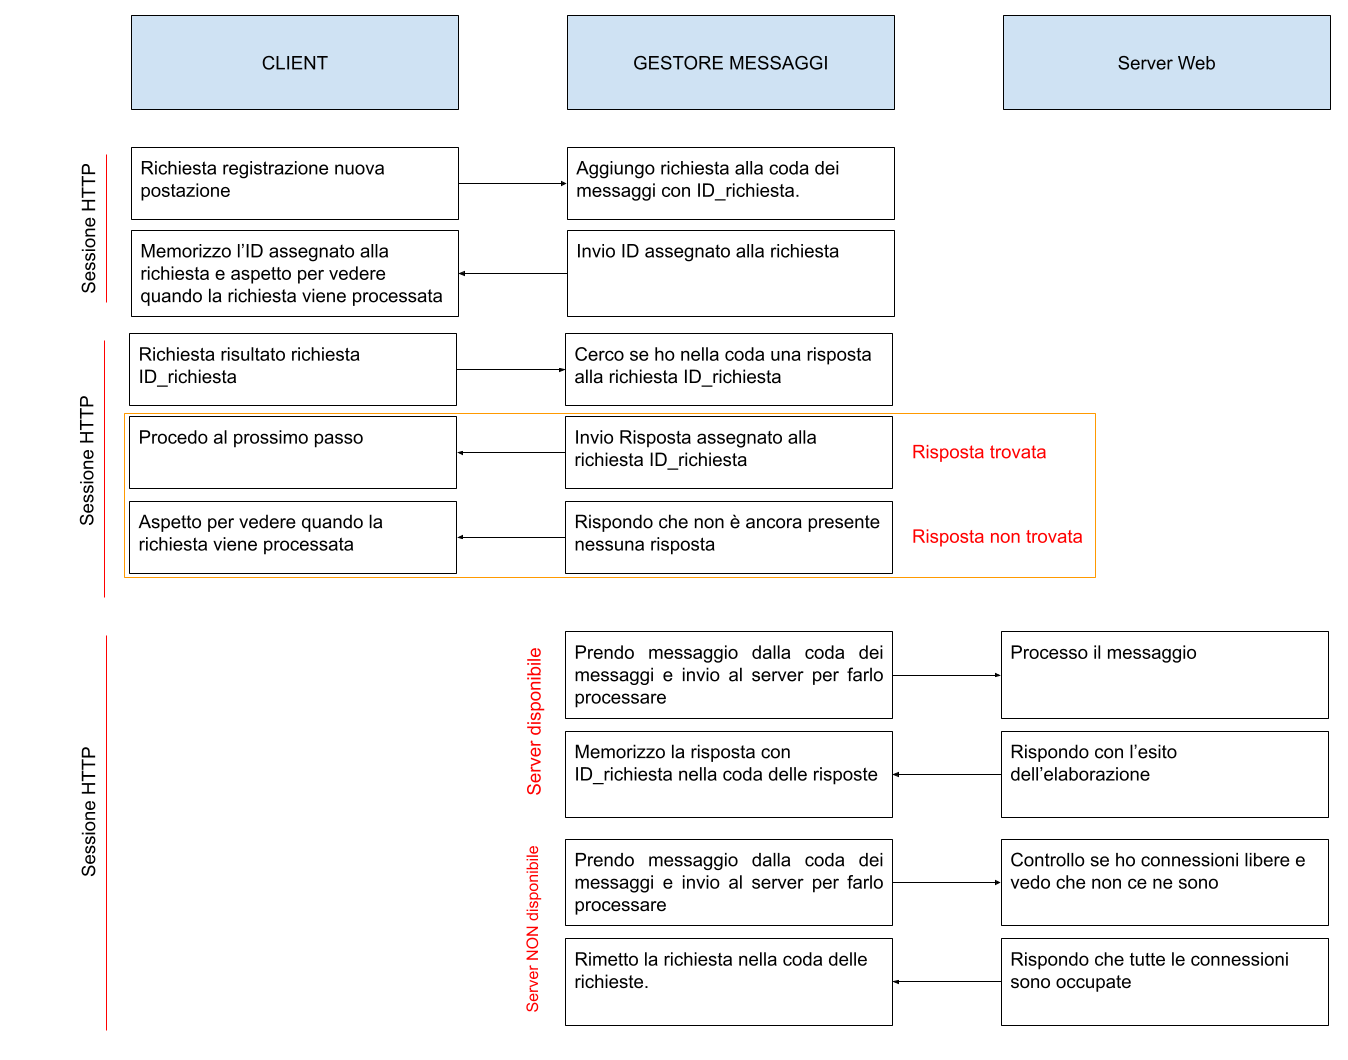
\includegraphics[width=1.0\textwidth]{figure/Disegno 004_ Esempio comunicazione con gestore messaggi}
	\caption{Esempio comunicazione con gestore messaggi}
	\label{fig:Esempio_comunicazione_con_gestore_messaggi}
\end{figure}


\section{Diagrammi degli stati}
Per comprendere meglio quali sono i messaggi che saranno necessari per la comunicazione con il server useremo dei diagrammi degli stati.

\begin{figure}[!hbtp]
	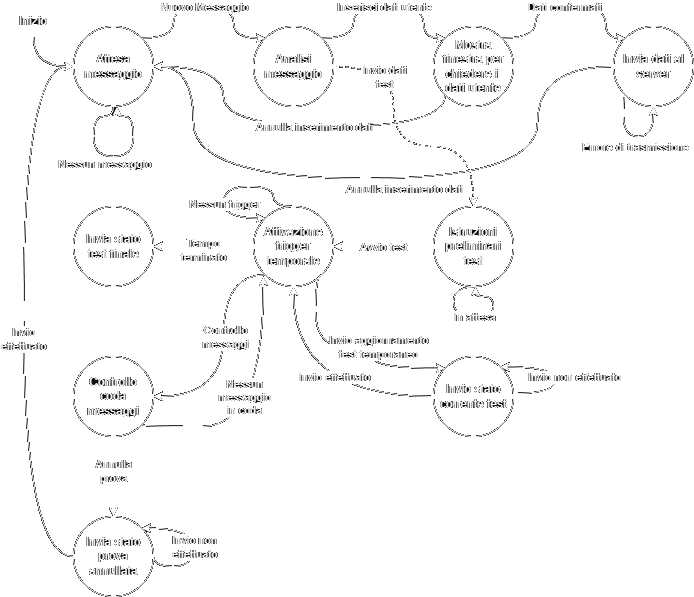
\includegraphics[width=1.0\textwidth]{figure/diagramma_degli_stati_client.png}
	\caption{Diagramma degli stati del Client}
	\label{fig:diagramma_stati_client}
\end{figure}

Sul client, per l'esecuzione di un test la sequenza delle operazioni che questo dovr\`a eseguire \`e la seguente:

\begin{enumerate}
	\item Registrazione postazione sul server PHP*
	\item Inserimento del codice della prova da svolgere nella pagina web da parte dell'utente
	\item Invio richiesta dati del test in base al codice inserito*
	\begin{itemize}
		\item Se il codice non \`e corretto scrivo Codice non corretto e lo faccio inserire di nuovo
		\item Se il codice \`e corretto usa i dati ricevuti dal server per creare dinamicamente la pagina web in base alle caratteristiche del test
	\end{itemize}
	\item Avvio i timer per lo svolgimento del test 
	\begin{itemize}
		\item Invio dello stato temporaneo del test (ogni 30s)*
		\item Controllo se ci sono messaggi o azioni richieste dal server ( interruzione test, messaggio a video, ecc.)*
	\end{itemize}
	\item Consegna test definitivo*
	\begin{itemize}
		\item Consegna manuale prima della scadenza
		\item Consegna per scadenza del tempo
	\end{itemize}
	\item Cancellazione registrazione della postazione*
\end{enumerate}
* vuol dire che c'\`e una richiesta HTTP

\section{Perch\'e scegliere Erlang}
Erlang \`e, come indicato anche nella pagina del progetto \cite{web:erlang}, un linguaggio usato per costruire sistemi soft real-time. massivamente scalabili con requisiti di alta disponibilit\`a. Alcuni dei suoi utilizzi riguardano le telecomunicazioni, il settore bancario, l'e-commerce, la telefonia computerizzata e la messaggistica istantanea. Il sistema di runtime di Erlang dispone di un supporto integrato per la concorrenza, la distribuzione e la tolleranza ai guasti.

Il motivo principale per cui l'ho scelto \`e la sua capacit\`a di scalare usando una quantit\`a minima di risorse. Inoltre pu\`o lavorare in modo distribuito su pi\`u macchine e pu\`o, in caso di errori nell'esecuzione del programma, ripristinare l'esecuzione in modo automatico.

\subsection{Erlang/OTP}
OTP che sta per Open Telecom Platform \`e un framework di sviluppo e una collezione di librerie, componenti di design e middleware che permettono di strutturare applicazioni Erlang in modo robusto e standardizzato.

OTP fornisce dei modelli pronti all'uso per gestire i compiti pi\`u comuni come ad esempio:
\begin{itemize}
	\item \textbf{gen\_server} - Per implementare la logica client-server
	\item \textbf{gen\_statem} - Per gestire macchine a stati finiti
	\item \textbf{supervisor} - Fondamentale per la tolleranza ai guasti (monitora altri processi e li riavvia se falliscono
\end{itemize}

Un concetto fondamentale di Erlang/OTP \`e l'albero di supervisione (\textit{supervision tree}). Questo \`e una modalit\`a di strutturazione del modello basato sull'uso di \textit{workers} e \textit{supervisors}.

\begin{itemize}
	\item I \textit{worker} sono i processi che svolgono effettivamente il lavoro.
	\item I Supervisori (\textit{supervisors}) sono processi che monitorano i \textit{worker} e fanno li fanno ripartire se ci sono problemi. 
\end{itemize}

L'albero di supervisione (\textit{supervision tree}) \`e una organizzazione gerarchica del codice in supervisori e worker che ci permette di progettare sistemi che sono resistenti ai guasti (\textit{fault-tolerant}).

\begin{figure}[!hbtp]
	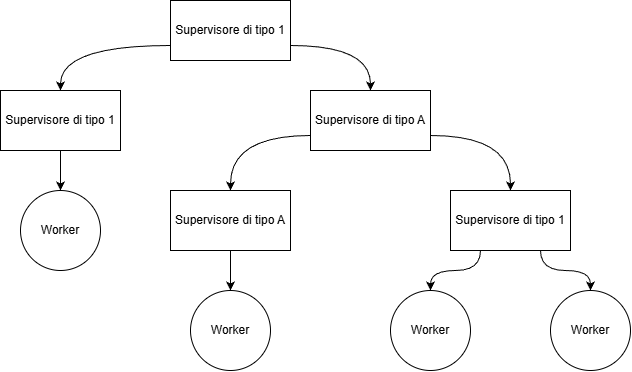
\includegraphics[width=1.0\textwidth]{figure/Erlang-OTP Supervision Tree.png}
	\caption{Supervision Tree}
	\label{fig:erlang-otp-supervision-tree}
\end{figure}

Una cosa molto interessante \`e che i supervisori e i worker possono essere sulla stessa macchina ma possono anche essere messi su macchine diverse. Questo ci permette di garantire che, anche se il problema riguarda fisicamente una macchina, il sistema pu\`o continuare a funzionare, creando nuovi nodi che svolgano i compiti che venivano svolti sulla macchina non pi\`u funzionante.

\subsection{Invio e ricezione di messaggi}
Altra caratteristica estremamente interessante di Erlang \`e la gestione nativa dei messaggi.

I vari processi (attori), infatti, possono comunicare tra di loro con un sistema di messaggistica nativo del linguaggio. Ad esempio per inviare un messaggio ad un altro processo \`e sufficiente il comando:

\begin{verbatim}
Pid ! Messaggio
\end{verbatim} 

Dove \textit{Pid} \`e l'id del processo a cui inviare il messaggio.

Per ricevere messaggi, un processo utilizza il blocco receive, che analizza la "cassetta postale" (mailbox) del processo stesso.

\begin{verbatim}
receive
    Pattern1 -> Azioni1;
    Pattern2 -> Azioni2
end
\end{verbatim} 

a seconda del \textit{pattern} ricevuto verr\`a eseguita l'azione corrispondente. 

\subsection{Hot Code Swapping}
Un'altra caratteristica interessante di erlang rispetto ad altri linguaggi \`e la sua capacit\`a di aggiornare il codice di una applicazione mentre questa \`e in esecuzione (\textit{Hot Code Swapping}), senza interrompere il servizio. I nuovi processi utilizzeranno il nuovo codice, mentre quelli vecchi continueranno con la versione precedente finch\`e non terminano o vengono aggiornati.


\subsection{Casi d'uso - Whatsapp}
Erlang \`e estremamente efficente e ne abbiamo prova, ad esempio, dal fatto che la gestione di messaggi dell'applicazione di messaggistica \textit{Whatsapp} viene fatta utilizzando le macchine virtuali BEAM di Erlang.

La capacit\`a di gestire una elevata concorrenza permette ad ogni server di gestire fino a 2 milioni di connessioni contemporanee. Questo gli permette, con un team estremamente ridotto, di gestire tranquillamente oltre 100 miliardi di messaggi al giorno mantenendo, grazie alla struttura \textit{fault-tolerant}, una enorme affidabilit\`a e tolleranza ai guasti.




